\documentclass[UTF8,a4paper]{ctexart}
%\usepackage[UTF8]{ctex}
\usepackage{graphicx}
\usepackage{url}
\usepackage{geometry}
\geometry{a4paper,scale=0.8}
\usepackage{setspace}
\setstretch{1.6}

\begin{document}
\begin{sloppypar}


	\begin{center}
	
\includegraphics[width = 14cm]{picture/s1}

		\begin{fontsize}{60pt}{20pt}
			实验报告
		\end{fontsize}

		\bigskip
		\bigskip
		
		\begin{fontsize}{20pt}{20pt}
			\begin{flushright}
				—— {\Huge Shell}与{\Huge Vim}的学习与应用
			\end{flushright}
		\end{fontsize}
		
		\bigskip
		\bigskip
		\bigskip
		\bigskip
		\bigskip
		\bigskip
		\bigskip
		\bigskip
		\bigskip
		\bigskip
		\bigskip
		\bigskip
		\bigskip
		\bigskip
		\bigskip
		\bigskip
		
		\begin{fontsize}{25pt}{20pt}

			学号:
			\underline{{\huge 23060021010}}
			\bigskip
			\bigskip
			\bigskip
			\bigskip

			姓名:
			\underline{郭晓伟}
			\bigskip
			\bigskip
			\bigskip
			\bigskip

			班级:
			\underline{{\Huge 23}级软件工程五八班}
				
		\end{fontsize}
	\end{center}
	\section{实验要求}
	\subsection{学习Shell和Vim的使用}
	\subsection{完成4个课堂练习与20个与Shell和Vim有关的实例}

			\bigskip
			\bigskip
			\bigskip
			\bigskip

	\section{实验内容}
	\subsection{Shell的学习}
	\subsubsection{Shell 是一种命令行解释器和脚本编写环境,主要用于与操作系统的内核进行交互。它作为用户与操作系统之间的接口,允许用户输入命令并执行系统功能。Shell 可以理解并执行用户输入的命令,将它们传递给操作系统的内核,然后将结果返回给用户。\\Shell 通常以文本的形式运行,可以通过命令行终端访问。在 UNIX 和类 UNIX 系统(如 Linux 和 macOS)中,shell 是一个非常重要的工具,它允许用户执行各种系统管理任务、文件操作、网络配置等。\\常见的Shell类型有Bash、Zsh、Fish、Csh、Ksh。}
	\subsubsection{Shell的主要功能:\\1.命令解释: 接受用户输入的命令并传递给操作系统执行。\\2.脚本编写: 通过编写 Shell 脚本,用户可以自动化一系列操作,比如文件管理、系统监控、任务调度等。\\3.变量管理: Shell 允许用户创建和使用变量,以便在脚本中存储和操作数据。\\4.管道与重定向: 通过管道将一个命令的输出作为另一个命令的输入,或者通过重定向 控制输入输出。\\5.进程管理: Shell 可以启动、停止、后台运行进程,并管理系统资源的分配。}
	\subsubsection{Bash的核心功能:\\变量和参数: 在 Bash 中,变量可以通过 = 进行赋值,使用时通过 \$ 符号引用。\\Bash 支持条件语句和循环,如if-else,for循环等。\\函数: 可以在 Bash 中定义和调用函数,以实现代码的复用和模块化。\\管道:通过 \textbar 将一个命令的输出传递给另一个命令。\\重定向:将命令输出重定向到文件。}
	
	\newpage
	
	\subsection{Vim的学习}
	\subsubsection{Vim(Vi Improved)是一个功能强大、广泛使用的文本编辑器,特别在程序员和系统管理员中很受欢迎。它是经典编辑器 Vi 的增强版,支持多种功能如语法高亮、插件扩展、脚本编写等。}
	\subsubsection{Vim的特点:\\1.模式编辑:正常模式(Normal mode):用于浏览和编辑文件。按键直接影响光标移动和文本操作。插入模式(Insert mode):用于插入文本,类似于其他常见文本编辑器的编辑模式。可视模式(Visual mode):选择文本块进行操作(如复制、删除)。命令模式(Command mode):通过键入 : 来输入各种命令(如保存、退出等)。
\\2.高效的键盘操作: Vim 强调通过键盘进行操作,减少对鼠标的依赖,从而提高编辑效率。每个按键或按键组合都对应着一个特定的操作。\\3.强大的插件支持: Vim 有丰富的插件生态,可以通过插件扩展各种功能,如代码补全、文件树导航、Git 集成等。\\4.多平台支持: Vim 可以运行在不同的操作系统上,如 Linux、macOS 和 Windows,因此它被广泛用于跨平台的文本编辑。\\5.轻量级与可定制性: Vim 的配置非常灵活,可以通过 .vimrc 文件定制编辑器的行为、外观和功能。}
	

	\bigskip
	\bigskip
	\bigskip
	\bigskip

	\section{实验中遇到的问题与解决方法}
	\subsection{使用Latex撰写实验报告时,发现编译出来的PDF文档中出现部分文字无法显示或显示不全的问题}
	原因是内容太多而 LaTeX 无法自动分页,使用newpag命令手动添加分页,即可显示全部文字。
	\subsection{在向仓库中提交敏感信息时,无法提交并显示who you are?}
	这是由于没有登记个人信息,在命令行终端输入指令git config --global user.email "邮箱"、git config --global user.name "名称",登记个人名称和邮箱之后即解决。
	\subsection{在使用Latex进行文本编辑时,无法显示中文}
	查阅资料后得知,Latex基础字体不包含中文,有两种方法,一为导入含有中文字体的宏包,二可以设置文章类型,采用经过国人开发的ctexbook、ctexart和ctexbeamer类型,这些类型自带了对中文的支持,且编译器要换成XeLaTex。
	\subsection{即使加入了graphicx宏包也无法插入图片}
	想要插入图片需要将图片放在与tex文件同一目录中,或者通过语句graphicspath引入图片所在的文件夹,用includegraphics语句来表示要插入的图片、设置图片的长宽。
	\subsection{完成文本写作后,结果第一页是空白页,文本内容从第二页开始}
	第一页默认为封面页,需要添加封面。
	
			\bigskip
			\bigskip
			\bigskip
			\bigskip
			
	\graphicspath{{picture/}}
	\section{实例练习}
	\subsection{创建Git仓库}
	输入git status命令,查看是否为仓库,并输入git init命令,初始化git仓库
	
	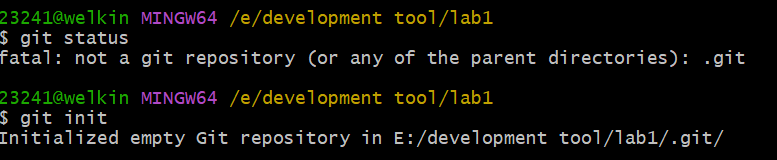
\includegraphics[width = 16cm]{1}
	
	\subsection{查看当前状态}
	输入git status指令,显示当前工作目录和暂存区的状态,提示仓库中有文件未追踪
	
	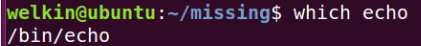
\includegraphics[width = 16cm]{2}
	
	\subsection{添加文件}
	git add "文件名",将文件添加到git仓库
	
	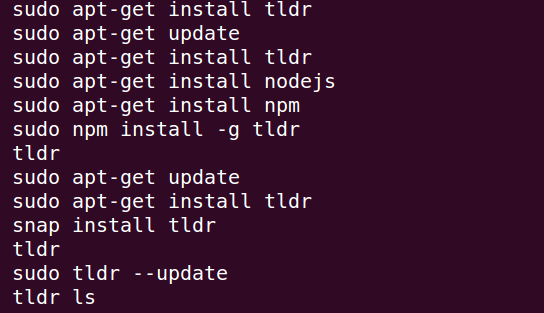
\includegraphics[width = 16cm]{3}
	
	\subsection{提交文件}
	git commit -m "提交信息",将文件提交到仓库中,并附上提交信息
	
	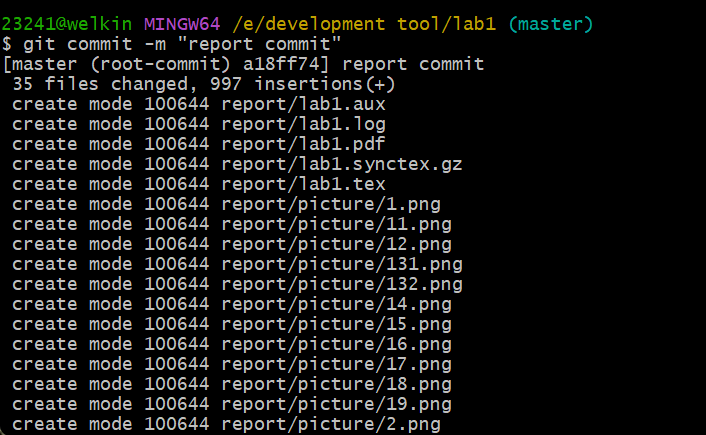
\includegraphics[width = 16cm]{4}
	
	\subsection{查看提交日志}
	git log,显示当前分支的提交历史,包括提交ID、作者、日期和提交信息
	
	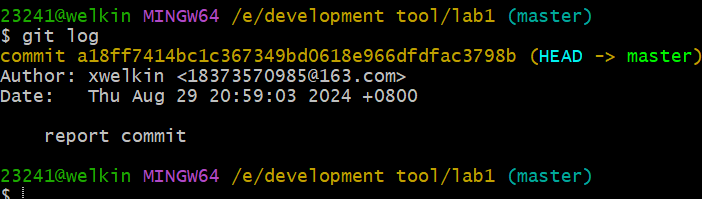
\includegraphics[width = 16cm]{5}
	
	\subsection{创建仓库分支并查看}
	git branch命令,查看 Git 仓库的分支情况,git branch a 则为创建一个名为a的分支,当前分支仍为主分支
	
	
\includegraphics[width = 16cm]{6}
	
	\subsection{切换分支}
	输入git checkout a命令,切换到a分支,也可以在创建分支的同时,直接切换到新分支,命令为git checkout -b
	
	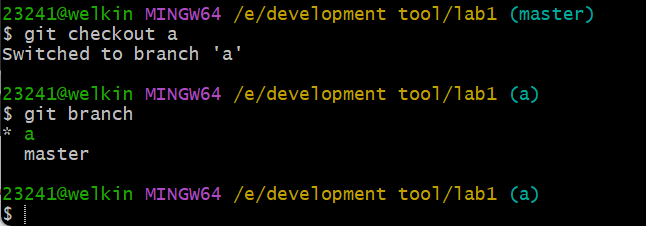
\includegraphics[width = 16cm]{7}
	
	\subsection{合并分支}
	切换到master分支,然后输入git merge a命令,将a分支合并到master分支
	
	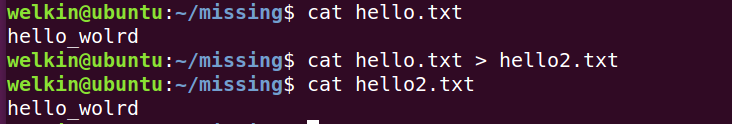
\includegraphics[width = 16cm]{8}
	
	\subsection{删除其他分支}
	输入git branch -d a命令,删除a分支。有时通过git branch -d命令出现删除不了的现象,例如分支a的代码没有合并到主分支等,这时可以通过命令git branch -D进行强制删除
	
	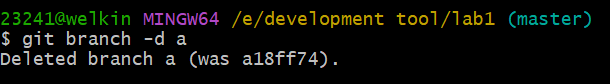
\includegraphics[width = 16cm]{9}
	
	\subsection{关联远程仓库}
	git remote add origin "远程仓库地址" 命令,关联远程仓库,其中origin为远程仓库的名字
	
	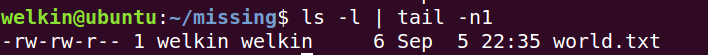
\includegraphics[width = 16cm]{10}
	
	\subsection{本地代码推到远程仓库}
	如果我们本地的代码有了更新,为了保持本地与远程的代码同步,我们就需要把本地的代码推到远程的仓库,使用git push origin master命令
	
	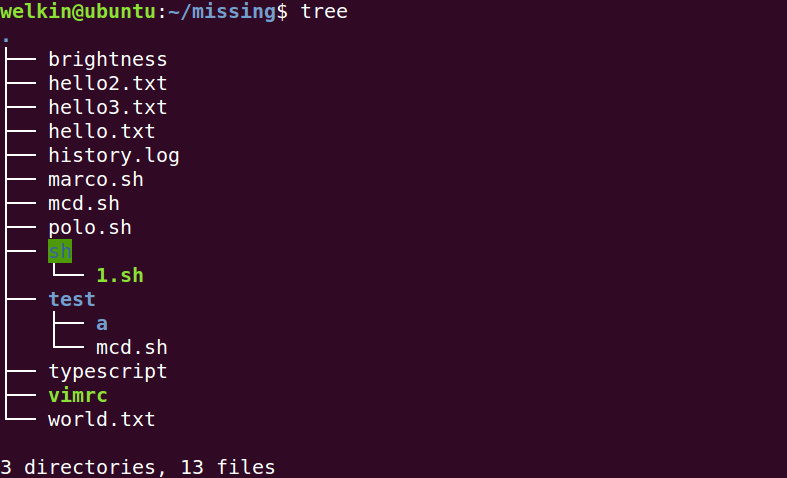
\includegraphics[width = 16cm]{11}
	
	\subsection{远程代码拉到本地}
	如果我们远程仓库的代码有了更新,同样为了保持本地与远程的代码同步,我们就需要把远程的代码拉到本地,使用git pull origin master命令
	
	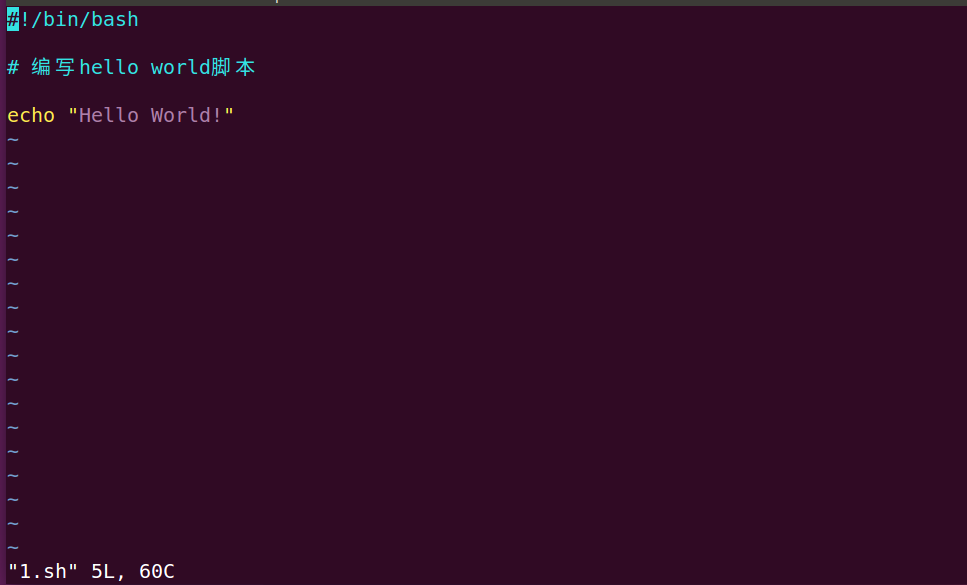
\includegraphics[width = 16cm]{12}
	
	\subsection{Latex实现中文}
	采用文章类型如经过国人开发的ctexbook、ctexart和ctexbeamer类型,自带中文支持,并且编译器换为XeLaTex
	
	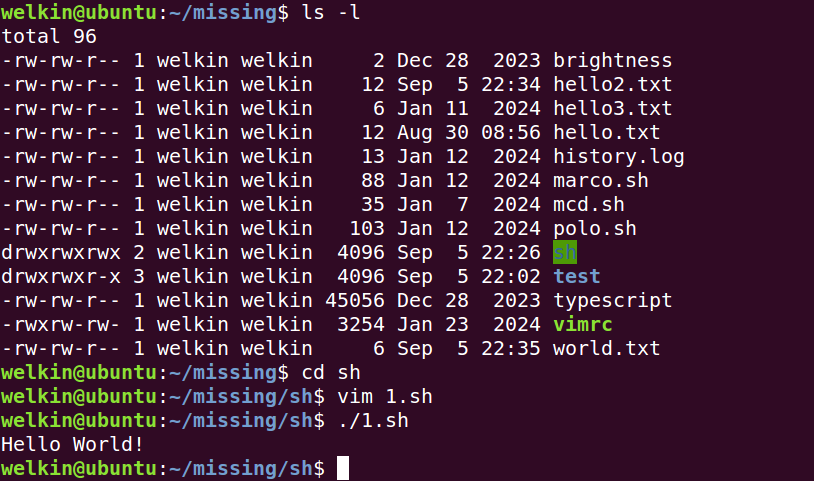
\includegraphics[width = 16cm]{13}
	
	\subsection{实现标题与作者等}
	可以用title、author、date来设置,日期中选择today会自动输出编译当天的日期。它们只能放在导言区,然后通过maketitle展现出来
	
	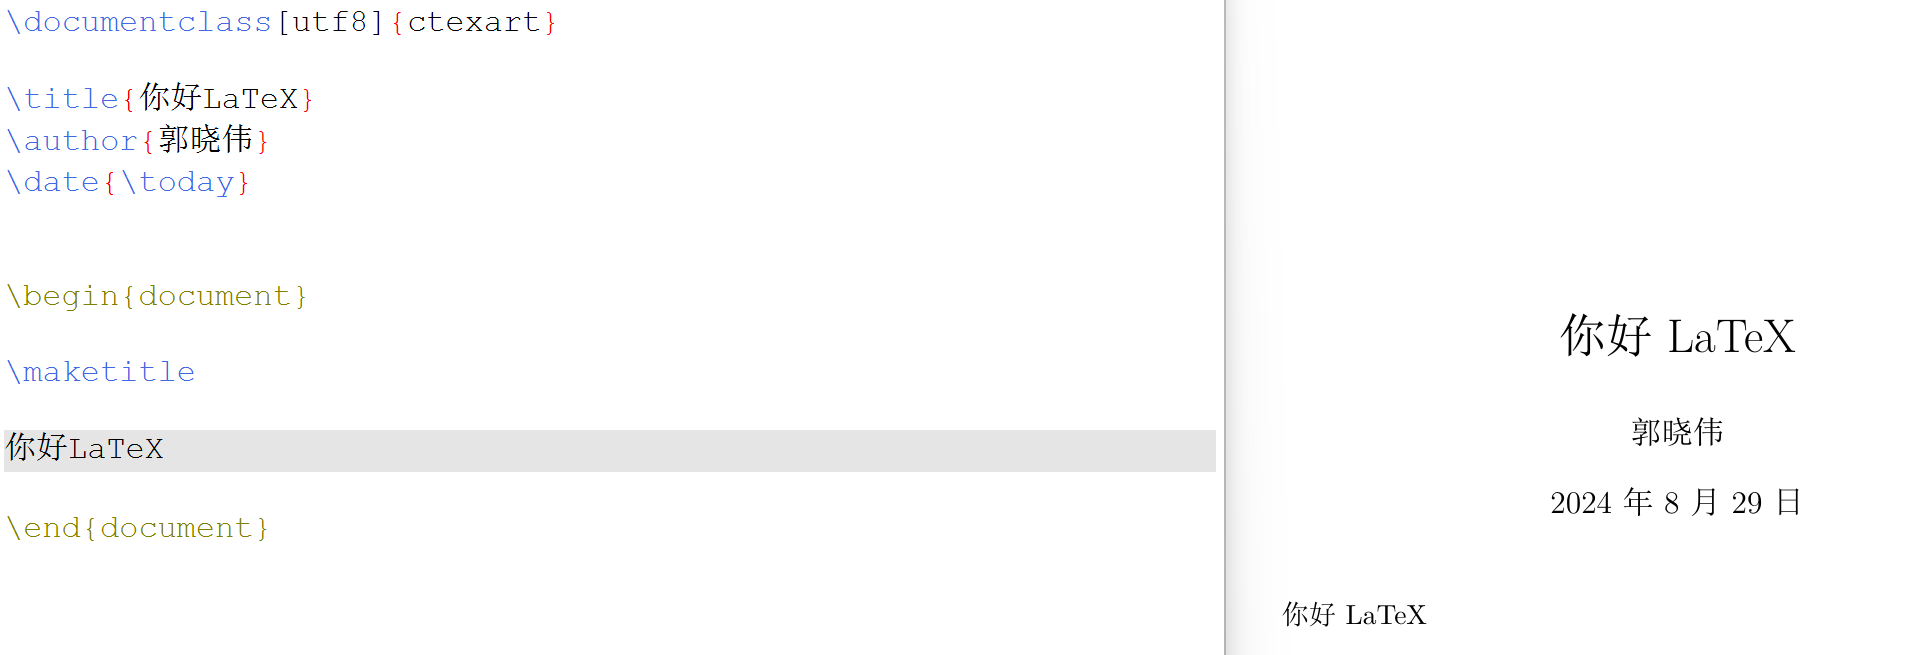
\includegraphics[width = 16cm]{14}
	
	\subsection{实现文章段落}
	章节分三阶,section、subsection、subsubsection,在它们后面的花括号中填写题目,加入*则可以消去前面对应的序数
	
	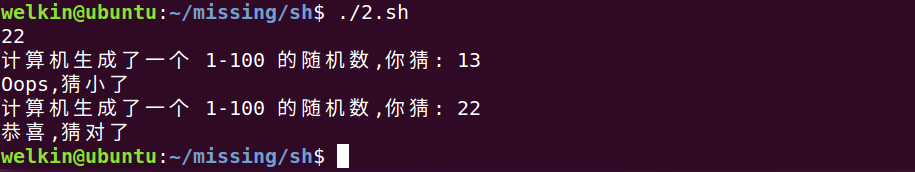
\includegraphics[width = 16cm]{15}
	
	\subsection{插入图片}
	插入图片需要使用graphicx宏包,使用includegraphics,可以在width=后设置宽度
	
	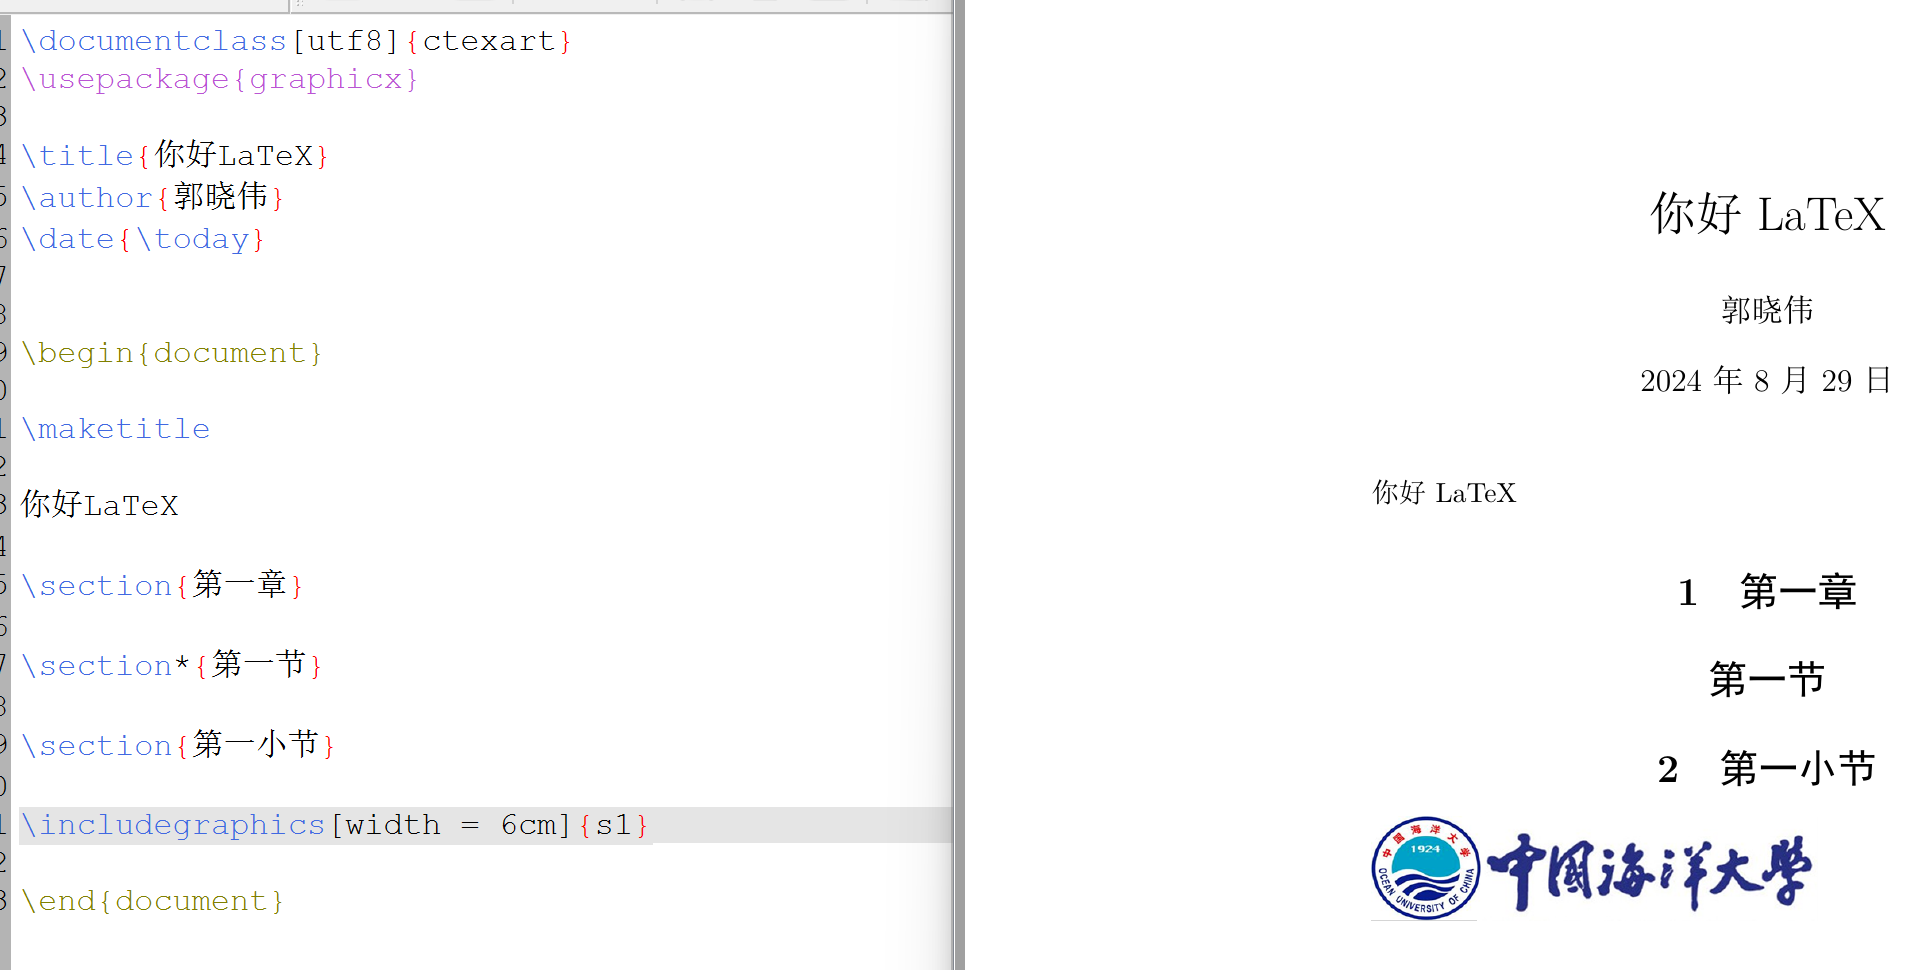
\includegraphics[width = 16cm]{16}
	
	\subsection{插入代码}
	调用listings宏包,并且在正文中使用lstlisting指令框住所想插入的代码,后面的中括号框内的语言选项帮助关键字高亮
	
	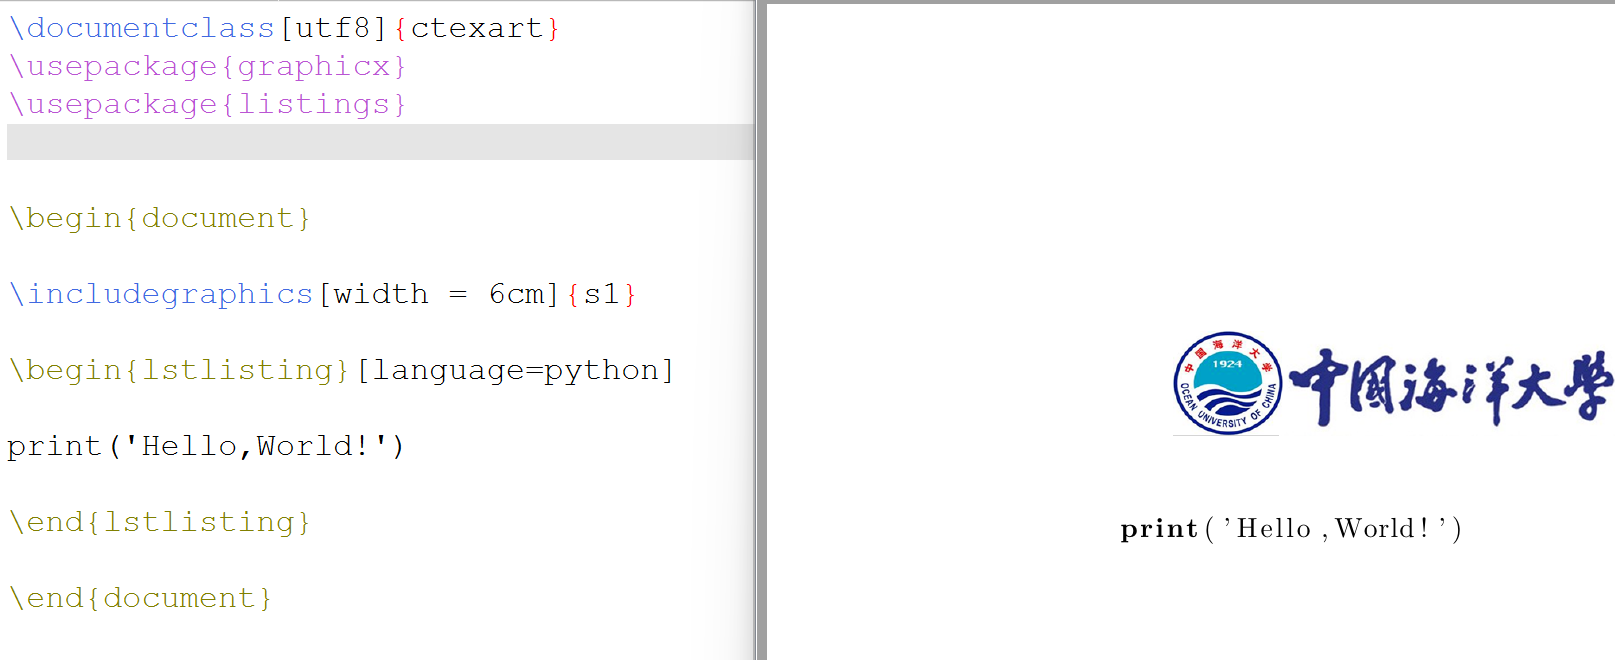
\includegraphics[width = 16cm]{17}
	
	\subsection{注释}
	Latex可以实现单行注释和多行注释
	
	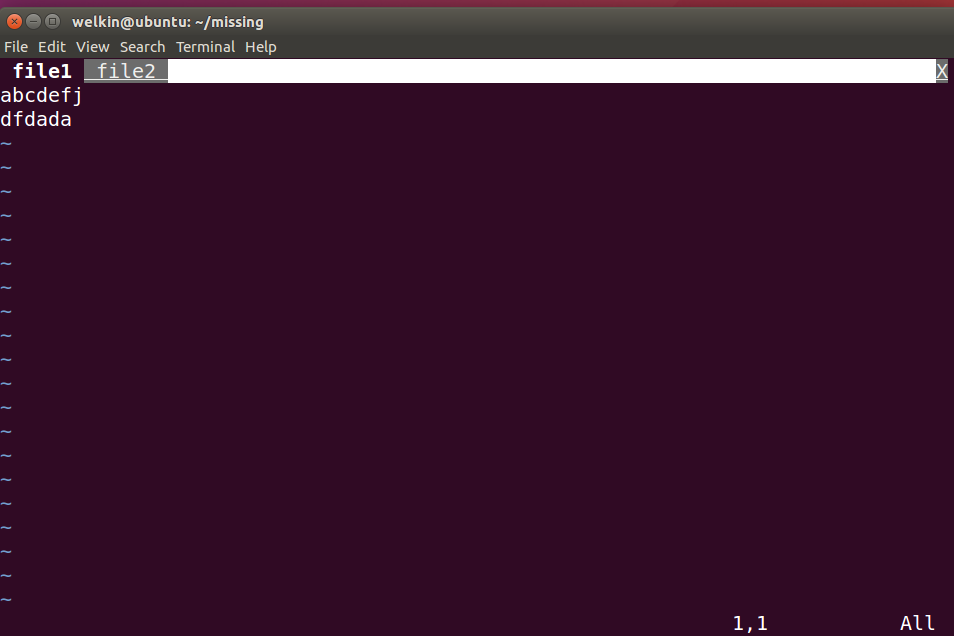
\includegraphics[width = 12cm]{18}
	
	\subsection{插入超链接}
	导入宏包url,使用url+链接
	
	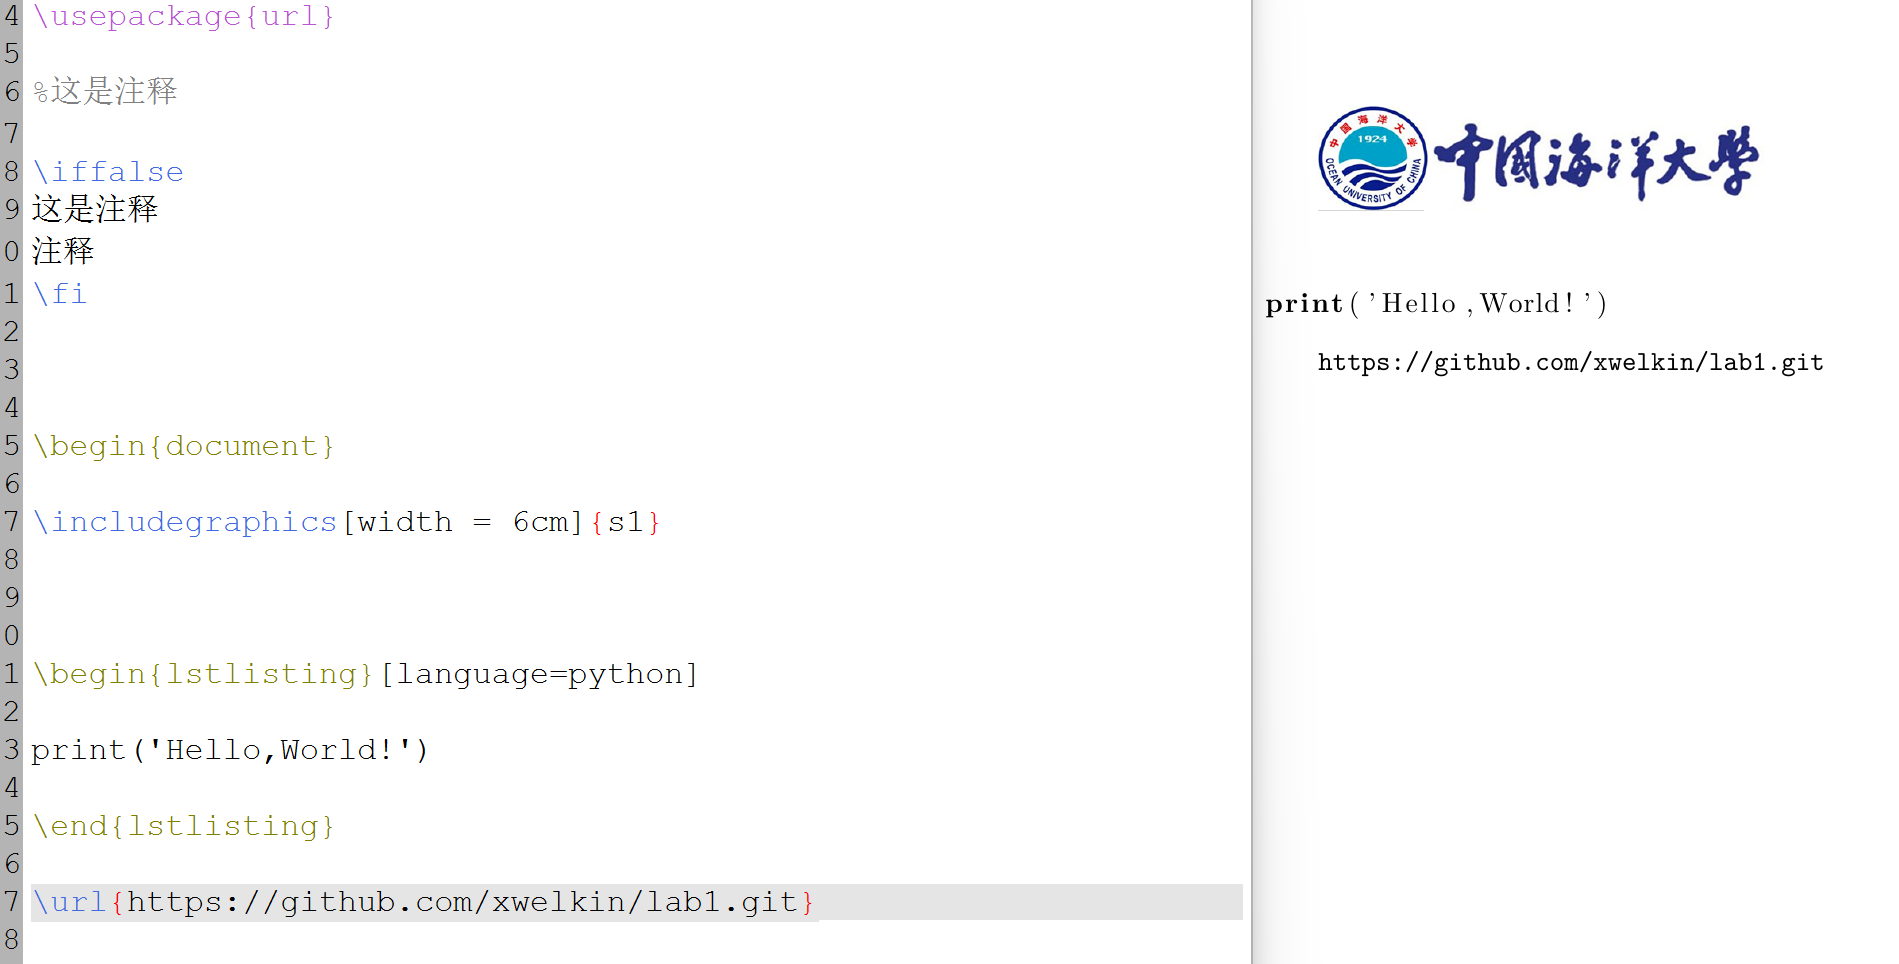
\includegraphics[width = 16cm]{19}
	
	\subsection{数学公式}
	输入数学公式需要导入宏包amsmath,使用equation
	
	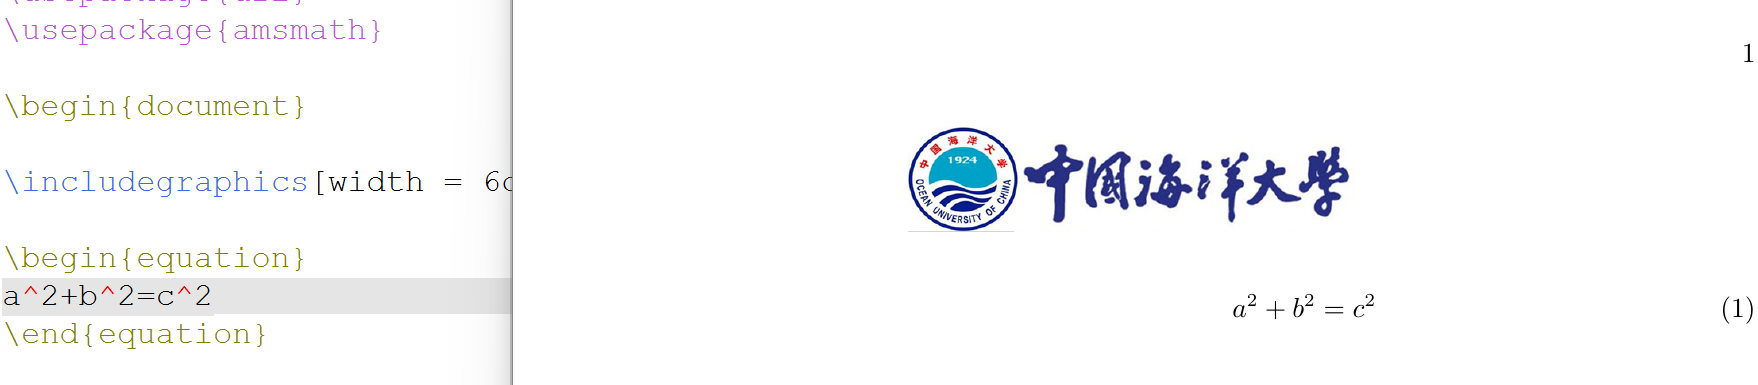
\includegraphics[width = 16cm]{20}

	\section{实验收获与感悟}
	通过学习Git和LaTeX,我深刻体会到版本控制在项目管理中的重要性。Git不仅能够有效记录和更改项目版本,还能帮助解决冲突。我掌握了Git的分支管理和合并技巧,明白了它在团队协作中作为沟通桥梁的重要作用,这能够大大减少沟通成本并提升工作效率。这次学习让我进一步适应了Git的独特工作方式和思维模式。\\
	\indent LaTeX凭借其卓越的排版能力,可以生成美观、专业的文档,尤其是其强大的数学公式编辑功能,能够轻松呈现复杂的数学表达式,提升论文的可读性并确保符合学术规范。此外,我还学会了如何在网上查找合适的论文模板,并将其tex文件移植过来,极大地提高了写论文的效率。这为我未来撰写数学建模比赛论文奠定了坚实基础。\\
	\indent 虽然学习Git和LaTeX的过程充满挑战,但它们带给我的收获和启发却是巨大的。Git让我掌握了版本控制和团队协作的核心要素,而LaTeX则让我能够以更专业和高效的方式编写文档。这两种工具不仅提升了我的技术能力,也让我更深入地理解了项目管理和学术研究的本质。我相信在未来的学习和工作中,它们将继续发挥重要作用,并为我提供有力的支持。\\
	
	Github仓库链接:\url{https://github.com/xwelkin/lab1.git}
	
\end{sloppypar}
\end{document}